\documentclass[12pt]{article}

\usepackage[utf8]{inputenc}
\usepackage{datetime}
\usepackage{amsthm}
\usepackage{amsmath}
\usepackage{amssymb}
\usepackage{enumitem}
\usepackage[USenglish]{babel}
\usepackage{matlab-prettifier}
\usepackage{graphicx}
\usepackage[makeroom]{cancel}
\usepackage{afterpage}
\usepackage{capt-of}

\DeclareMathOperator*{\argmin}{arg\,min}
\DeclareMathOperator*{\argmax}{arg\,max}

\newcommand\independent{\protect\mathpalette{\protect\independenT}{\perp}}
\def\independenT#1#2{\mathrel{\rlap{$#1#2$}\mkern2mu{#1#2}}}

\newtheoremstyle{colon}{\topsep}{\topsep}{}{}{\bfseries}{:}{ }{}
\theoremstyle{colon}
\newtheorem{exercise}{Exercise}
\newtheorem*{answer}{Answer}

\title{ORFE 525: Statistical Learning and \\ Nonparametric Estimation \\ Homework 4}
\author{Zachary Hervieux-Moore}

\newdate{date}{18}{04}{2017}
\date{\displaydate{date}}

\begin{document}

\maketitle

\clearpage

\begin{exercise}
  In this problem, we will be using K-means clustering on Wiki\-pedia introductions of famous individuals who are associated with Princeton University. Through our analysis, we will determine broad categories that capture the different academic and cultural backgrounds of these individuals. This analysis is part of the field called ``topic modeling''.

  \begin{enumerate}[label=\arabic*)]
    \item Load in the dataset \texttt{Wikipedia.RData}. Print out the head of the dataset. Who are the first 3 individuals in the dataset and their corresponding professions? (It's okay to give a broad category). Then use the script \texttt{script1\_HW4.R} to convert the matrix into a term-document matrix. How many individuals are there? How many words are there? What are the top 10 most frequent words in the entire dataset? List the 0\%, 25\%, 50\%, 75\%, and 100\% quantiles of the word counts across the entire dataset. The phenomenon you will see can be attributed to ``Zipf's Law'', saying the distribution of word counts in any text data follows an exponential-like curve. In the later questions, we will like to handle these ``over-represented'' words.

    \item We notice that the top ten words are not very interesting with ``the'' and ``and'' being among the most frequent words. One way to combat this is to re-parameterize the matrix. Use the script \texttt{script2\_HW.R} to use the \texttt{tf-idf} parametrization (common in text-analysis). Based on this new \texttt{tf-idf} parameterization, what are the 10 words with highest total weight across the entire dataset?

    \item Great! Hopefully we are starting to see meeaningful topics appear, but the \texttt{tf-idf} parameterization might not be highly interpretable as our \texttt{dtm.mat} matrix containing the weights instead of word ounts. We would sitll like to know which words are common in the dataset (for our downstream analysis) but we'll like to remove ``common'' words. Run the scripts \texttt{script3\_HW4.R}, which does the following two things: First, it removes words that appear too frequently across all the documents. For example, the word ``Princeton'' is in every document. Second, it removes the top 300 most frequent words according to Google.

      After running the script, how many words are left in our analysis? What are the top ten words in our remaining \texttt{dtm.mat.raw}?

    \item We see that the most common words in \texttt{dtm.mat.raw} are now similar to the top-weighted words in \texttt{dtm.mat}. This is great for our future interpretability. Now, let's zoom in on one particular person and make sure our data was processed correctly. Search for ``Ben Bernanke'' in our dataset. Print out the raw text for him according to \texttt{dat} (our original dataset). Find in this text the 10 top-weighted words according to \texttt{dtm.mat} and the 10 words with the highest word counts according to \texttt{dtm.mat.raw}.

    \item We will now implement K-means analysis. One of the most important ingredients for K-means is a good distance function. Typically, the Euclidean distance is used between two vectors, but in this question, we will assume that the cosine-distance is more appropriate (\texttt{https://en.{ }wikipedia.org/wiki/Cosine\_similarity}). We will work with the \texttt{dtm.mat} (the \texttt{tf-idf} parameterized) matrix when we use K-means (as it includes all the words), but we will use \texttt{dtm.mat.raw} to interpret our results (as it includes only the important words we want to see).

      Renormalize all the columns of \texttt{dtm.mat} to have norm 1. Then using \texttt{norm.sim.ksc} in the \texttt{akmeans} package, set the seed to 10 (for reproducibility) and find 8 clusters according to \texttt{dtm.mat}. How big are each of the resulting clusters? Based on the cluster assignments, print out the top 25 words in each cluster according to \texttt{dtm.mat.raw}. Also, print out the quantiles (0\%, 25\%, 50\%, 75\%, 100\%) of the word counts with non-zero word counts within each cluster to get a send of how significant the top words are.
  \end{enumerate}
\end{exercise}

\begin{answer}
  All code for this question is in the appendix below.
  \begin{enumerate}[label=\arabic*)]
    \item The first 3 individuals are shown in Table 1.
      \begin{center}
        \captionof{table}{Profession}
        \begin{tabular}{ c | c }
          Individual & Profession \\
          \hline
          Michel Che & Chemist \\
          Hossein Modarressi & Jurist \\
          Xiao-Gang Wen & Physicist
        \end{tabular}
      \end{center}
      There are 812 individuals and 6889 words. The top 10 most frequent words are
      \begin{center}
        ``the'', ``and'', ``univers'', ``for'', ``was'', ``his'', ``from'', ``has'', ``with'', ``new''
      \end{center}
      The quantiles are in Table 2.
      \begin{center}
        \captionof{table}{Quantiles for Word Frequency}
        \begin{tabular}{ c | c | c | c | c}
          0\% & 25\% & 50\% & 75\% & 100\% \\
          \hline
          2 & 3 & 5 & 14 & 17317
        \end{tabular}
      \end{center}

    \item Based on the new parametrization, the 10 words with the most weight are
      \begin{center}
        ``she'', ``her'', ``music'', ``econom'', ``law'', ``scienc'', ``mathemat'', ``new'', ``histori'', ``research''
      \end{center}

    \item After running the script, the number of words left is 6633 and the top ten words are
      \begin{center}
        ``she'', ``her'', ``histori'', ``econom'', ``polit'', ``law'', ``music'', ``mathemat'', ``theori'', ``physic''
      \end{center}

    \item The raw text for Ben Bernanke is:

      ben shalom bernanke brnki brnangkee born december 13 1953 is an american economist at the brookings institution who served two terms as chairman of the federal reserve the central bank of the united states from 2006 to 2014 during his tenure as chairman bernanke oversaw the federal reserves response to the late2000s financial crisisbefore becoming federal reserve chairman bernanke was a tenured professor at princeton university and chaired the department of economics there from 1996 to september 2002 when he went on public service leavefrom 2002 until 2005 he was a member of the board of governors of the federal reserve system proposed the bernanke doctrine and first discussed the great moderation the theory that traditional business cycles have declined in volatility in recent decades through structural changes that have occurred in the international economy particularly increases in the economic stability of developing nations diminishing the influence of macroeconomic monetary and fiscal policybernanke then served as chairman of president george w bushs council of economic advisers before president bush nominated him to succeed alan greenspan as chairman of the united states federal reserve his first term began february 1 2006 bernanke was confirmed for a second term as chairman on january 28 2010 after being renominated by president barack obama his second term ended february 1 2014 when he was succeeded by janet yellen

      The top 10 weighted words in \texttt{dtm.mat} in this text are
      \begin{center}
        ``bernank'', ``reserv'', ``chairman'', ``feder'', ``term'', ``bush'', ``succeed'', ``econom'', ``janet'', ``volatil''
      \end{center}
      The highest word counts in \texttt{dtm.mat.raw} in this text are
      \begin{center}
        ``chairman'', ``bernank'', ``feder'', ``reserv'', ``term'', ``econom'', ``bush'', ``februari'', ``second'', ``succeed''
      \end{center}

    \item The size of the clusters are in Table 3
      \begin{center}
        \captionof{table}{Size of Clusters}
        \begin{tabular}{ c | c | c | c | c | c | c | c | c}
          cluster & 1 & 2 & 3 & 4 & 5 & 6 & 7 & 8 \\
          \hline
          size & 64 & 71 & 55 & 205 & 117 & 52 & 109 & 139
        \end{tabular}
      \end{center}

      \clearpage

      The top words by cluster are in Table 4
      \begin{center}
        \captionof{table}{Top Words by Cluster}
        \begin{tabular}{ c | c | c | c }
          1 & 2 & 3 & 4 \\
          \hline
          ``she''       & ``physic''    & ``she''    & ``she''        \\
          ``econom''    & ``theori''    & ``her''    & ``polit''      \\
          ``her''       & ``mathemat''  & ``team''   & ``econom''     \\
          ``histori''   & ``she''       & ``coach''  & ``law''        \\
          ``academi''   & ``her''       & ``play''   & ``her''        \\
          ``theori''    & ``field''     & ``band''   & ``program''    \\
          ``develop''   & ``prize''     & ``season'' & ``board''      \\
          ``physic''    & ``academi''   & ``their''  & ``polici''     \\
          ``comput''    & ``theoret''   & ``music''  & ``affair''     \\
          ``mathemat''  & ``quantum''   & ``assist'' & ``educ''       \\
          ``law''       & ``music''     & ``record'' & ``histori''    \\
          ``advanc''    & ``contribut'' & ``head''   & ``former''     \\
          ``technolog'' & ``develop''   & ``high''   & ``committe''   \\
          ``california''& ``string''    & ``jersey'' & ``social''     \\
          ``engin''     & ``known''     & ``album''  & ``offic''      \\
          ``geolog''    & ``comput''    & ``citi''   & ``develop''    \\
          ``polit''     & ``philosophi''& ``theolog''& ``journal''    \\
          ``press''     & ``histori''   & ``histori''& ``appoint''    \\
          ``then''      & ``then''      & ``career'' & ``secur''      \\
          ``area''      & ``use''       & ``design'' & ``washington'' \\
          ``had''       & ``california''& ``game''   & ``foundat''    \\
          ``join''      & ``engin''     & ``had''    & ``join''       \\
          ``use''       & ``mani''      & ``hockey'' & ``elect''      \\
          ``astronomi'' & ``under''     & ``began''  & ``assist''     \\
          ``career''    & ``general''   & ``more''   & ``dure''
        \end{tabular}
        \begin{tabular}{ c | c | c | c }
          5 & 6 & 7 & 8 \\
          \hline
          ``music''     & ``histori''   & ``she''       & ``she''        \\
          ``she''       & ``polit''     & ``her''       & ``her''        \\
          ``her''       & ``her''       & ``histori''   & ``law''        \\
          ``team''      & ``she''       & ``econom''    & ``then''       \\
          ``play''      & ``modern''    & ``literatur'' & ``board''      \\
          ``polit''     & ``philosophi''& ``mathemat''  & ``play''       \\
          ``perform''   & ``war''       & ``review''    & ``develop''    \\
          ``histori''   & ``econom''    & ``journal''   & ``human''      \\
          ``orchestra'' & ``visit''     & ``editor''    & ``career''     \\
          ``festiv''    & ``california''& ``englisn''   & ``washington'' \\
          ``academi''   & ``european''  & ``law''       & ``name''       \\
          ``record''    & ``german''    & ``theolog''   & ``team''       \\
          ``econom''    & ``yale''      & ``critic''    & ``use''        \\
          ``mathemat''  & ``academi''   & ``languag''   & ``foundat''    \\
          ``theori''    & ``their''     & ``teach''     & ``into''       \\
          ``compos''    & ``advanc''    & ``write''     & ``mani''       \\
          ``symphoni''  & ``press''     & ``taught''    & ``were''       \\
          ``prize''     & ``germani''   & ``cultur''    & ``won''        \\
          ``london''    & ``historian'' & ``theori''    & ``academi''    \\
          ``visit''     & ``physic''    & ``press''     & ``citi''       \\
          ``ensembl''   & ``recent''    & ``former''    & ``had''        \\
          ``physic''    & ``under''     & ``human''     & ``but''        \\
          ``law''       & ``comput''    & ``music''     & ``histori''    \\
          ``press''     & ``later''     & ``prize''     & ``journal''    \\
          ``program''   & ``law''       & ``articl''    & ``servic''
        \end{tabular}
      \end{center}

      \clearpage

      The quantiles for each cluster are in Table 5
      \begin{center}
        \captionof{table}{Cluster Quantiles}
        \begin{tabular}{ c | c | c | c | c | c }
          cluster & 0\% & 25\% & 50\% & 75\% & 100\% \\
          \hline
          1 & 1 & 1 & 2 & 4 & 80 \\
          2 & 1 & 1 & 2 & 4 & 110 \\
          3 & 1 & 1 & 2 & 4 & 89 \\
          4 & 1 & 1 & 2 & 6 & 223 \\
          5 & 1 & 1 & 2 & 4 & 234 \\
          6 & 1 & 1 & 2 & 4 & 51 \\
          7 & 1 & 1 & 2 & 4 & 144 \\
          8 & 1 & 1 & 2 & 5 & 110
        \end{tabular}
      \end{center}
  \end{enumerate}

  \textbf{Code Appendix:}

  \begin{lstlisting}[language=R, basicstyle=\scriptsize, breaklines=true]
    # Part 1.1
    library(tm)
    library(XML)
    library(Matrix)
    library(slam)
    library(SnowballC)
    library(akmeans)
    library(lsa)

    ## First three names
    dataset <- local(get(load("./Wikipedia.RData")))
    dataset[1:3,"name"]

    ## Script 1
    text = dataset[,"text"]
    text = iconv(text, to = "utf-8") #some conversion on SMILE needed
    corpus = Corpus(VectorSource(text))
    dtm.control.raw <- list(tolower = TRUE, removePunctuation = TRUE, removeNumbers = TRUE,
                        removestopWords = TRUE, stemming = TRUE, wordLengths = c(3, 15), bounds = list(global = c(2, Inf)))

    dtm.raw = DocumentTermMatrix(corpus, control = dtm.control.raw)
    dtm.mat.raw = as.matrix(dtm.raw) # our term-document matrix

    ## Number of individuals and words
    print("Number of individuals:")
    dim(dtm.mat.raw)[1]

    print("Number of words:")
    dim(dtm.mat.raw)[2]

    ## 10 most frequent words
    words.sum <- colSums(dtm.mat.raw)
    words <- order(words.sum, decreasing = T)[1:10]
    print("The most common words are:")
    colnames(dtm.mat.raw)[words]

    ## Quantiles
    print("The quantiles are:")
    quantile(words.sum, probs = c(0,0.25,0.5,0.75,1))

    # Part 1.2

    ## Script 2
    dtm.control <- list(tolower = TRUE, removePunctuation = TRUE, removeNumbers = TRUE,
                        removestopWords = TRUE, stemming = TRUE, wordLengths = c(3, 15), bounds = list(global = c(2, Inf)),
                        weighting = function(x){weightTfIdf(x, normalize = FALSE)})

    dtm = DocumentTermMatrix(corpus, control = dtm.control)
    dtm.mat = as.matrix(dtm)

    ## 10 most frequent words
    words.sum <- colSums(dtm.mat)
    words <- order(words.sum, decreasing = T)[1:10]
    print("The most common words are:")
    colnames(dtm.mat)[words]

    # Part 1.3

    ## Script 3
    dtm.mat.indicator = dtm.mat.raw
    dtm.mat.indicator[dtm.mat.indicator!=0] = 1

    word.presence = apply(dtm.mat.indicator, 2, sum)
    idx = which(word.presence >= quantile(word.presence, prob = 0.99))
    dtm.mat.raw = dtm.mat.raw[,-idx]

    common.words = read.csv("google-10000-english.txt", header = F)
    idx = which(colnames(dtm.mat) %in% common.words[1:300,1])
    dtm.mat.raw = dtm.mat.raw[,-idx]

    ## How many words left
    print("Number of words left:")
    dim(dtm.mat.raw)[2]

    ## 10 most frequent words
    words.sum <- colSums(dtm.mat.raw)
    words <- order(words.sum, decreasing = T)[1:10]
    print("The most common words are:")
    colnames(dtm.mat.raw)[words]

    # Part 1.4

    ## Original data
    ben.id <- which(dataset$name == "Ben Bernanke")
    dataset[ben.id, "text"]

    ## Top ten in dtm.mat
    words <- order(dtm.mat[ben.id,], decreasing = T)[1:10]
    colnames(dtm.mat)[words]

    ## Top ten in dtm.mat.raw
    words <- order(dtm.mat.raw[ben.id,], decreasing = T)[1:10]
    colnames(dtm.mat.raw)[words]

    # Part 1.5

    ## Renormalize
    dtm.mat.norm <- t(quick.norm(t(dtm.mat), mod=1))

    ## Set set and run k means
    set.seed(10)
    print("Size of clusters:")
    k_means <- norm.sim.ksc(dtm.mat.norm, k=8)
    k_means$size

    ## Top 25 words in each cluster
    for (i in 1:8){
      words.sum <- colSums(dtm.mat.raw[which(k_means$cluster == i),])
      words <- order(words.sum, decreasing = T)[1:25]
      print(paste("Cluster ", i, ":", sep=""))
      print(colnames(dtm.mat.raw)[words])
    }

    ## Quantiles
    for (i in 1:8){
      words.sum <- colSums(dtm.mat.raw[which(k_means$cluster == i),])
      words.sum <- words.sum[words.sum > 0]
      print(paste("Cluster ", i, " quantiles:", sep=""))
      print(quantile(words.sum, probs = c(0,0.25,0.5,0.75,1)))
    }
  \end{lstlisting}
\end{answer}

\clearpage

\begin{exercise}
  In this problem, we are going to use images of 20 Miss Daegu 2013 contestants. The Korean beauty pageant caused some debates on plastic surgery since all the contestants look almost identical. We hope to rigorously analyze the data by PCA and try to visualize the similarities of those contestants. We get the 20 images from the candidates of that competition. The cropped and aligned images can be downloaded from Blackboard. We use function \texttt{readPNG} in R package \texttt{png} to load the images and get 20 arrays of dimensions $800 \times 580 \times 3$, where $800 \times 580$ is the total pixels of each image and 3 denotes RGB's 3 channels, each with a value ranging between 0 and 1. We only consider the face region of row pixel 171 to 400 and column pixel 206 to 375, then stack them together column by column to generate a $20 \times 117300$ matrix, and finally apply PCA.
  \begin{enumerate}[label=\arabic*)]
    \item \textbf{Solving PCA:} Let $X = (X_1, \mathellipsis, X_n)^T$ be the centered $n$ by $p$ data matrix where $X_i$ of length $p$ represents the information of the $i^{th}$ image. Here $n = 20$, $p = 117300$. PCA actually is equivalent to the diagonalization of sample covariance matrix $S = n^{-1} X^T X$. To be specific, left
      \begin{gather*}
        S = \frac{1}{n} X^T X = V \Lambda V^T
      \end{gather*}
      where $V = (v_1, \mathellipsis, v_p)$ is orthonormal and $\Lambda = \text{diag}(\lambda_1, \mathellipsis, \lambda_p)$ is diagonal with non-increasing elements. Let us assume distinct eigenvalues, i.e., $\lambda_i \neq \lambda_j$ for $i \neq j \leq n$. Note, $\lambda_i = 0$ for $i > n$. Calculating the eigendecomposition could be expensive due to the large number of $p$. We consider instead the decomposition,
      \begin{gather*}
        \frac{1}{n} X X^T = U D U^T
      \end{gather*}
      where $U = (u_1, \mathellipsis, u_n)$ is orthonormal and $D = \text{diag}(d_1, \mathellipsis, d_n)$ is diagonal with non-increasing elements. Prove $\lambda_i = d_i$ and $v_i = \frac{X^T u_i}{\sqrt{n \lambda_i}}$ for $i \leq n$. Use this fact in your coding to significantly improve efficiency to computer eigendecompositions.

    \item \textbf{Graphical Analyses:} Run PCA on the data matrix. Report the following plots and comment on your observations.
      \begin{itemize}
        \item Plot 1: Graph of PCA eigenvalues in decreasing order.
        \item Plot 2: Visualize the largest 6 eigenfaces by using function \texttt{write\-PNG}. Note that you need to first rescale eigenvectors into the region $[0,1]$ and create the corresponding array of dimension $230 \times 170 \times 3$.
        \item Plot 3: Define the coefficients of the $i^{th}$ image onto the $k^{th}$ eigenface as $\eta_{ik} = v_k^T X_i$. Note again $X_i$ is centered. Visualize the 20 images by plotting the coefficients corresponding to the first two eigenfaces.
        \item Plot 4: Define pairwise similarity of contestants $i$ and $j$ by $s_{ij} = \sum_{k=1}^6 (\eta_{ik} - \eta_{jk})^2$. For contestant $i$, by summing up $s_{ij}$ over $j$, we can get a measure of how the contestant is different from the rest. Plot $\sum_j s_{ij}$ vs contestant number $i$ and identify the 3 most salient contestants.
      \end{itemize}
  \end{enumerate}
\end{exercise}

\begin{answer}
  All code for this question is in the code appendix below.
  \begin{enumerate}[label=\arabic*)]
    \item First we note that
      \begin{gather*}
        \frac{1}{n} X X^T u_i = d_i u_i \\
        \frac{1}{n} X^T X X^T u_i = d_i X^T u_i
      \end{gather*}
      Thus, $X^T u_i$ is an eigenvector of $\frac{1}{n} X^T X$ with eigenvlaue $d_i$. However, we must normalize this eigenvector. We get that the norm is,
      \begin{gather*}
        u_i^T X X^T u_i = n \cdot d_i
      \end{gather*}
      Thus, we must divide by $\sqrt{n d_i}$. So we conclude that $v_i = \frac{X^T u_i}{\sqrt{n d_i}}$. However, since we now have an orthonormal eigenvector of $S$, we must have $d_i = \lambda_i$. So we conclude that $v_i = \frac{X^T u_i}{\sqrt{n \lambda_i}}$.

    \item The eigenvalue in decreasing order are shown in Figure 1. Values range from 56,600 to close to 10. Note the exponential decrease in size of the eigenvalues. That means that the first eigenvalue is incredibly explanatory of the variance.
      \begin{center}
        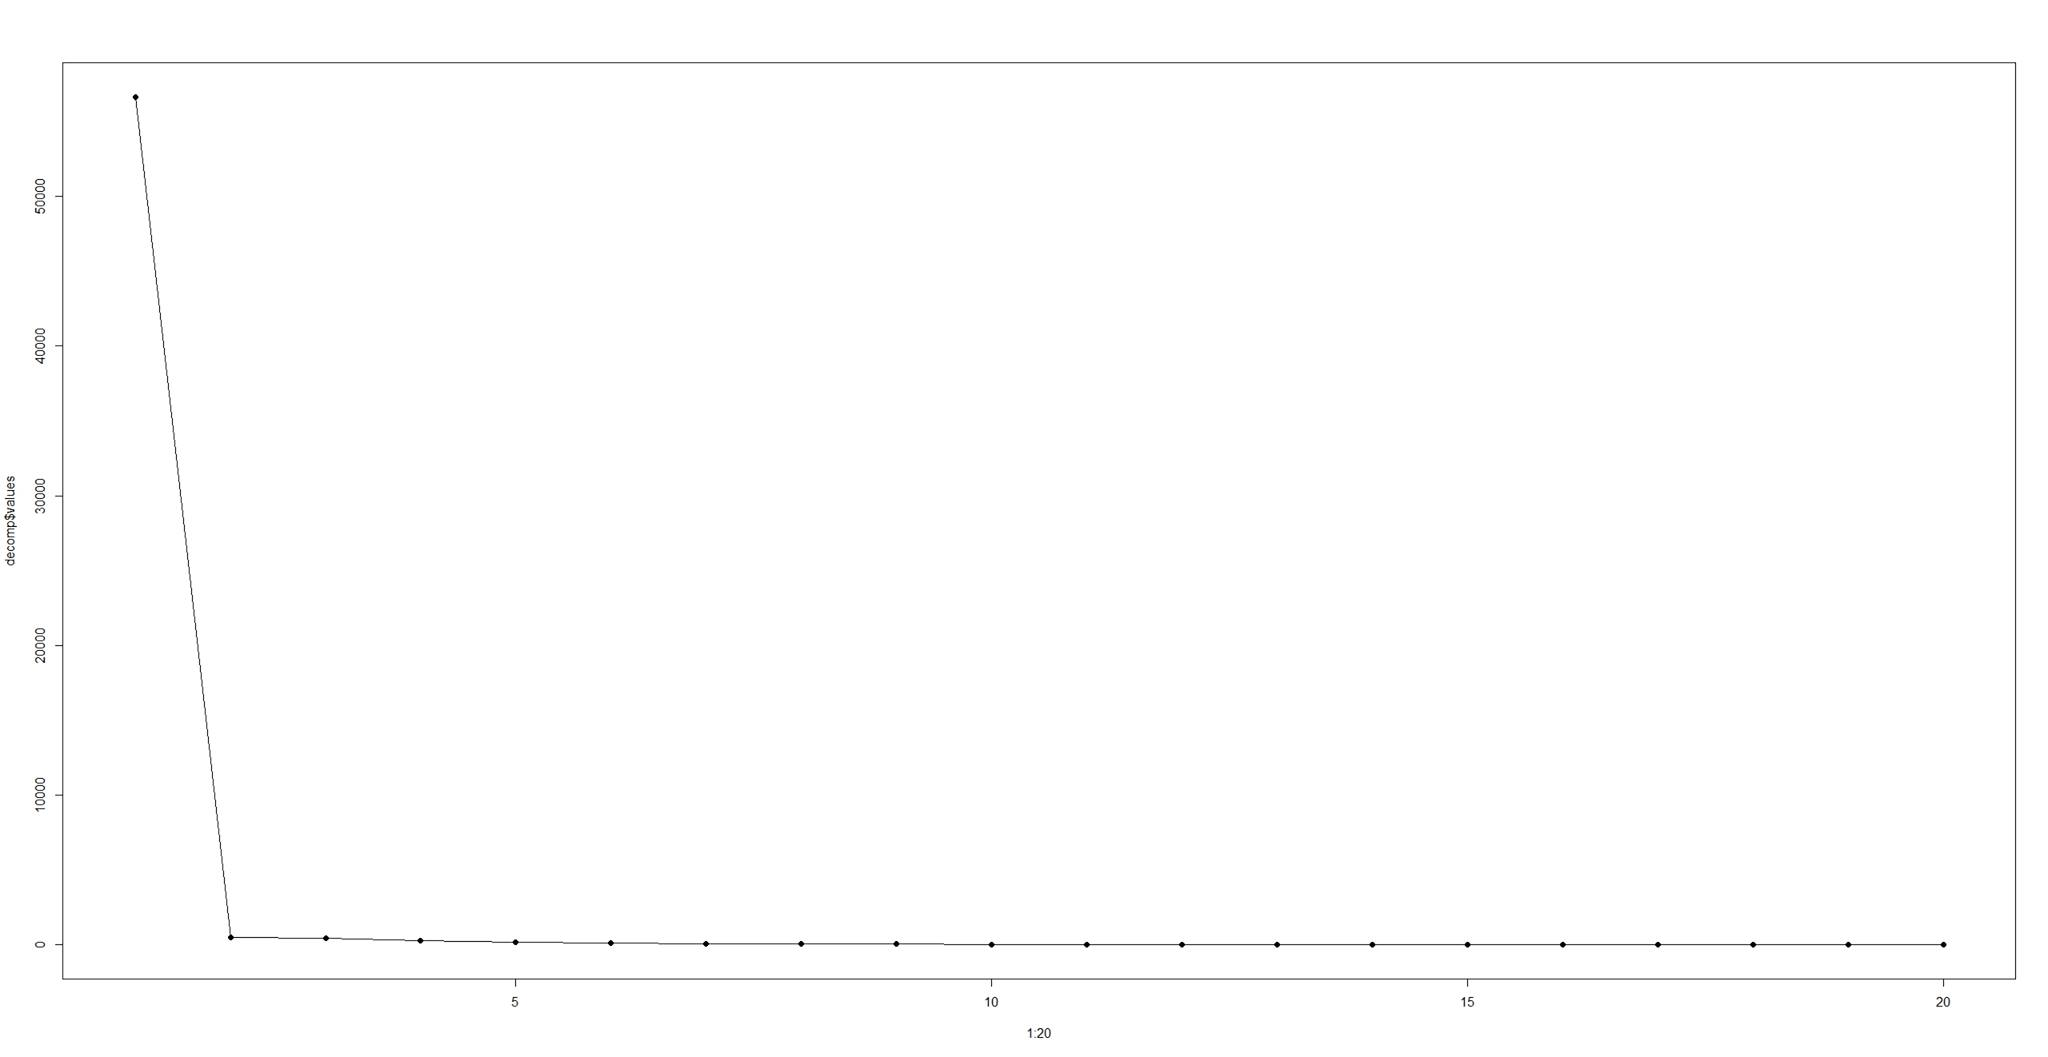
\includegraphics[width=0.9\textwidth]{eigenvalues.jpg}
        \captionof{figure}{PCA Eigenvalues}
      \end{center}

      The 6 largest eigenfaces are shown in Figure 2.
      \begin{center}
        
\includegraphics[width=0.3\textwidth]{eigenface1.png}
        
\includegraphics[width=0.3\textwidth]{eigenface2.png}
        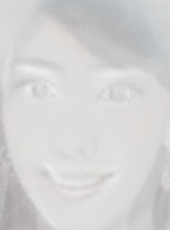
\includegraphics[width=0.3\textwidth]{eigenface3.png}
        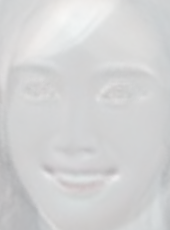
\includegraphics[width=0.3\textwidth]{eigenface4.png}
        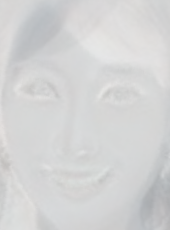
\includegraphics[width=0.3\textwidth]{eigenface5.png}
        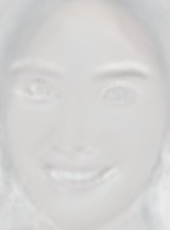
\includegraphics[width=0.3\textwidth]{eigenface6.png}
        \captionof{figure}{Six Largest Eigenfaces}
      \end{center}

      Figure 3 plots $\eta_{i1}$. The values range from -3200 to -4000. This is because the first eigenface is negative. This is obvious by looking at Figure 2 and seeing that it is black. Figure 4 shows $\eta_{i2}$. The values range from -700 to 700.
      \begin{center}
        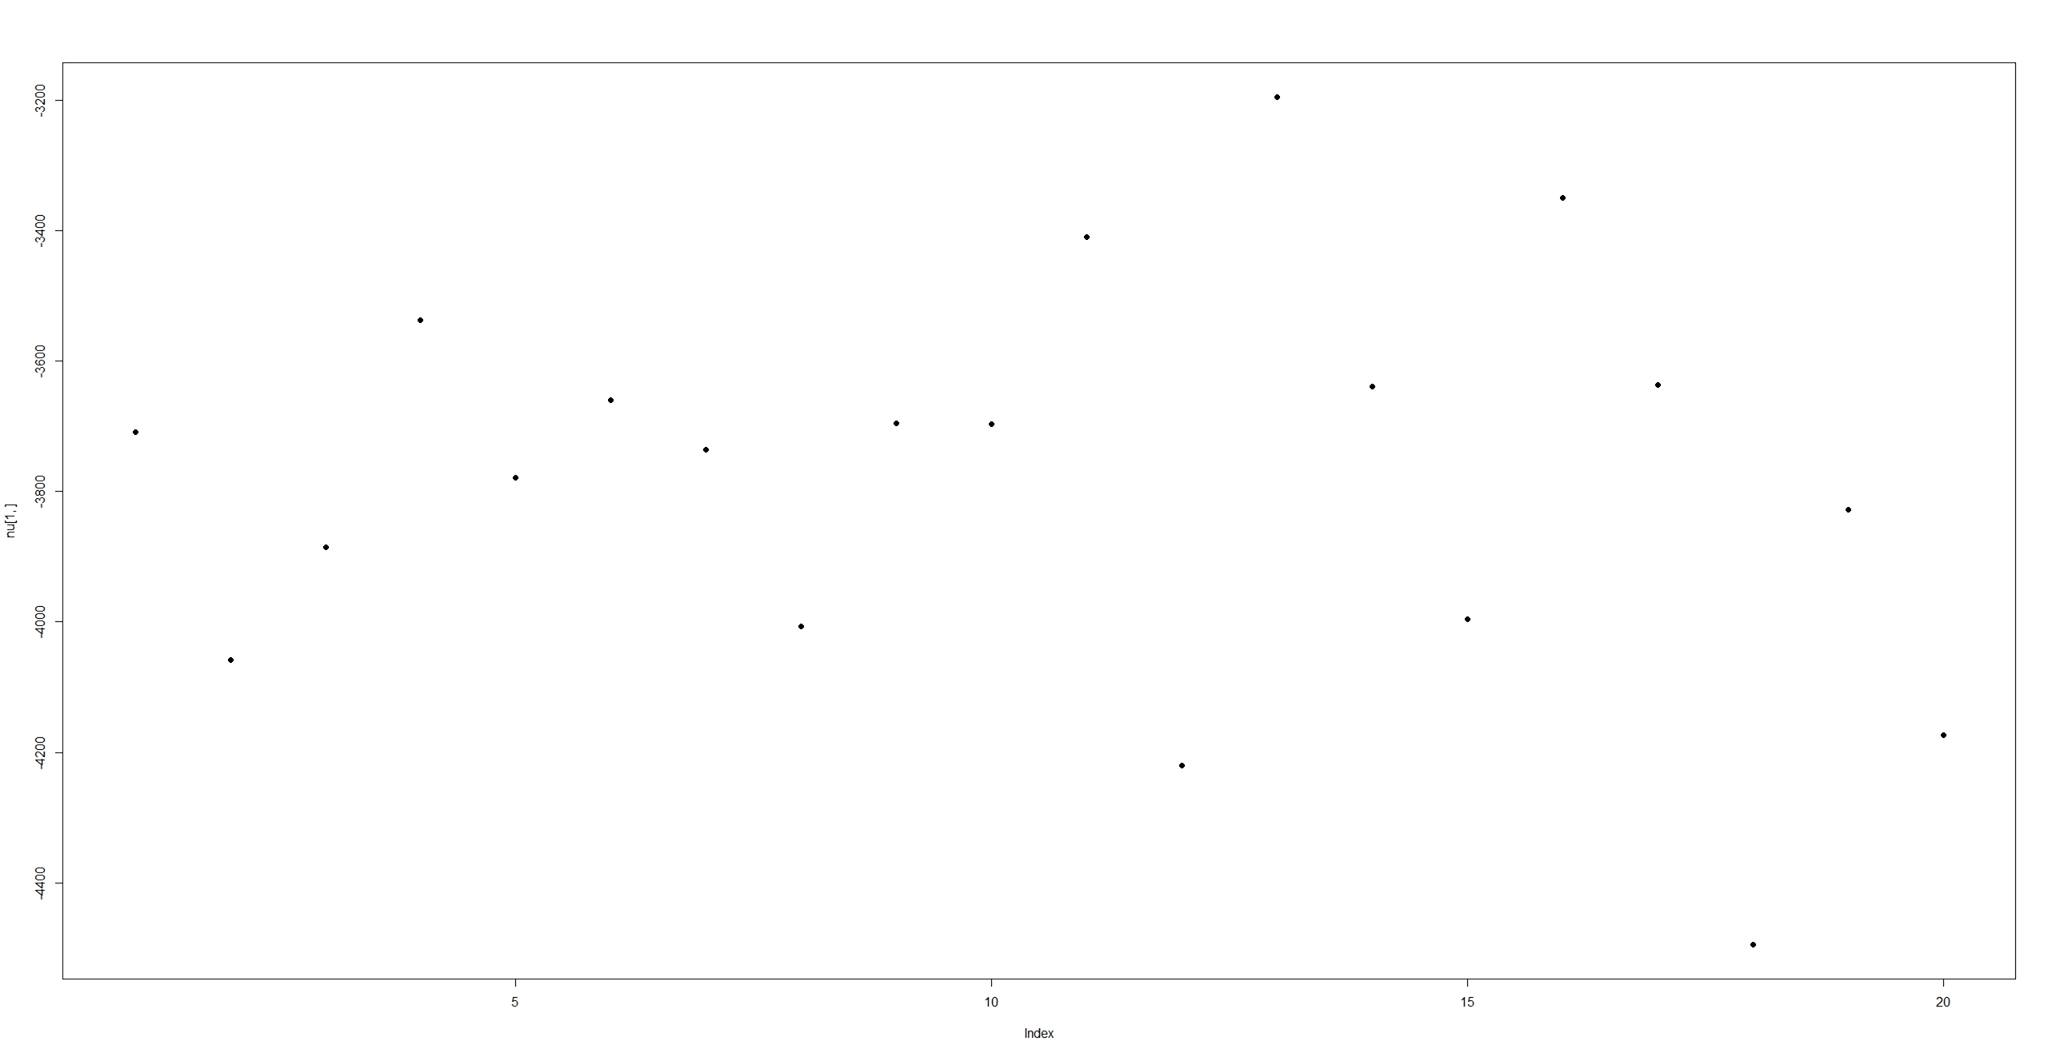
\includegraphics[width=0.9\textwidth]{eta_1.jpg}
        \captionof{figure}{$\eta_{i1}$ for all Contestants}
      \end{center}

      \begin{center}
        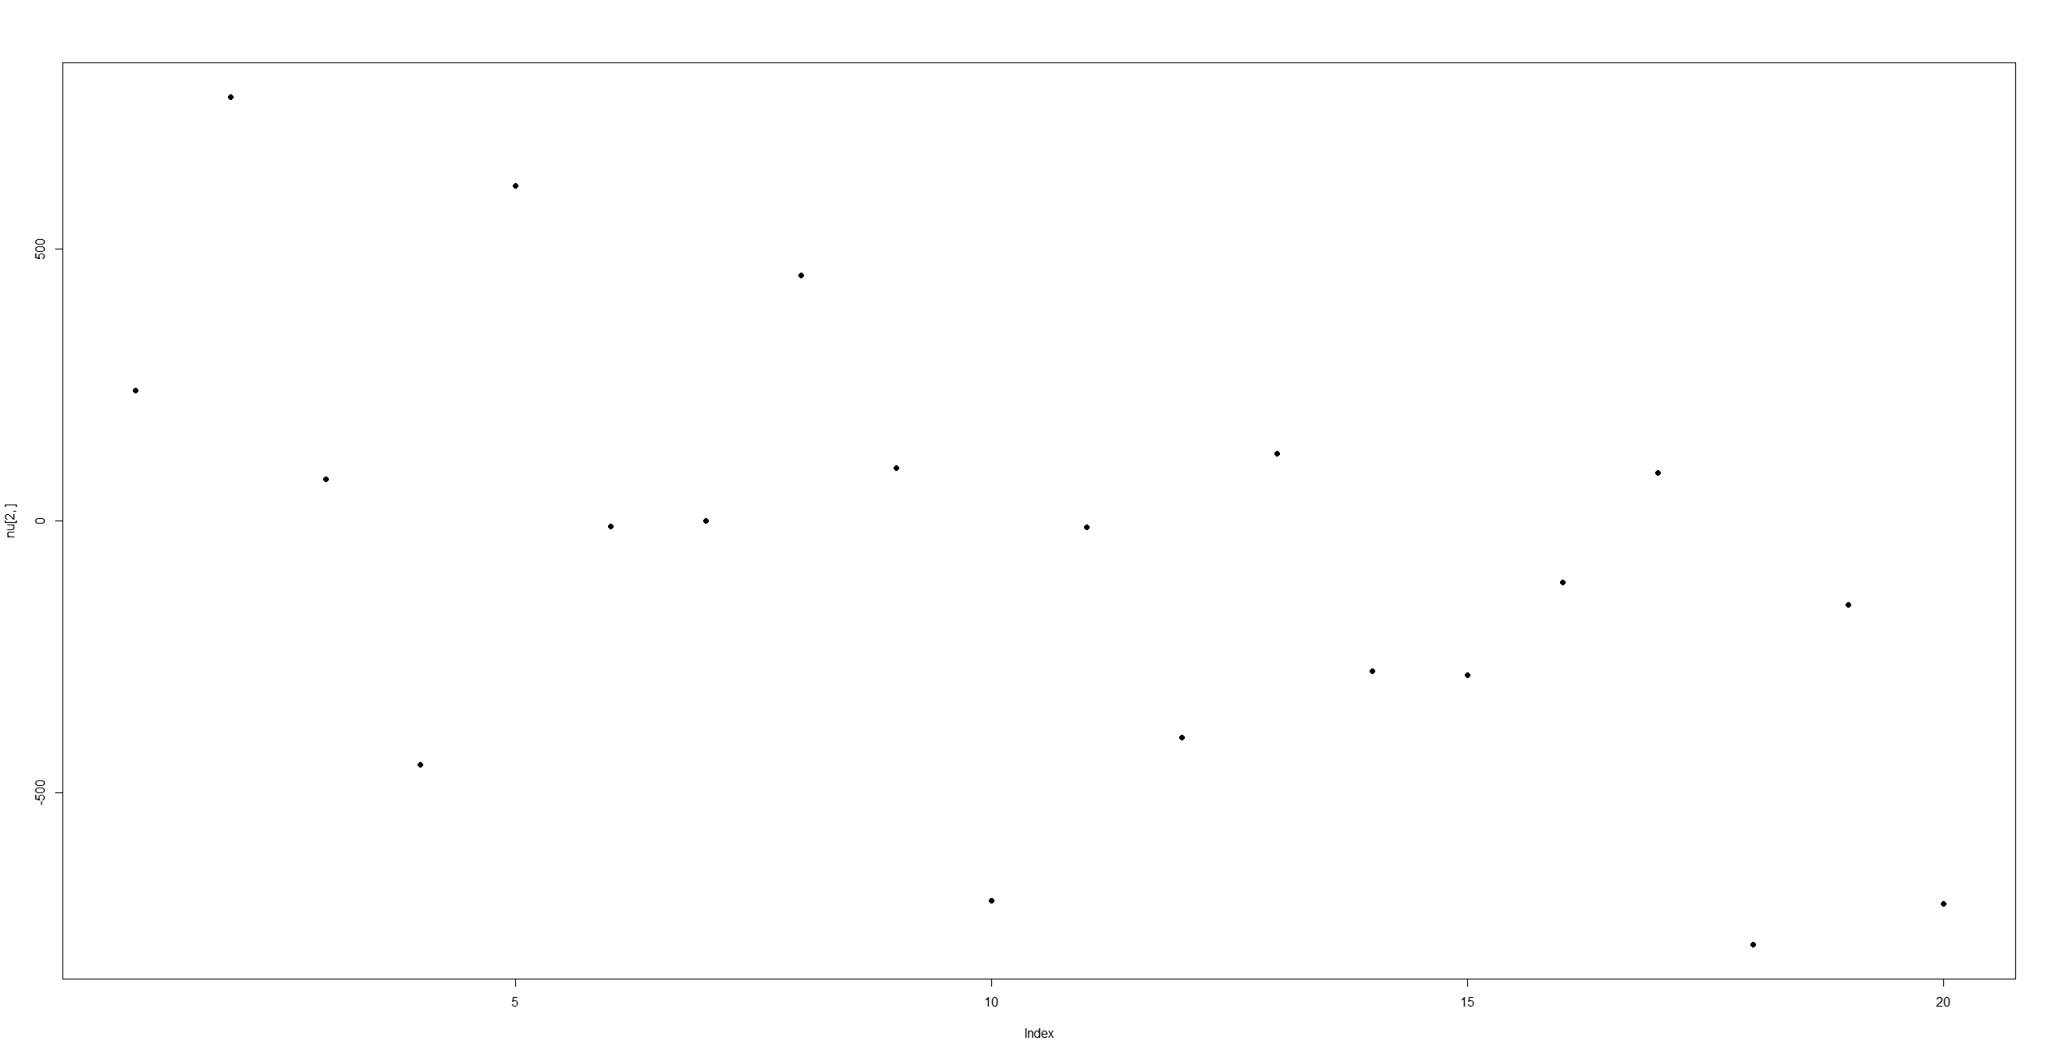
\includegraphics[width=0.9\textwidth]{eta_2.jpg}
        \captionof{figure}{$\eta_{i2}$ for all Contestants}
      \end{center}

      Figure 5 shows the Plot 4. Values range from $1.5e07$ to $3.5e07$. Note that the vast majority of them are roughly equal in similarity to the rest. Also, they are all the same order of magnitude
      \begin{center}
        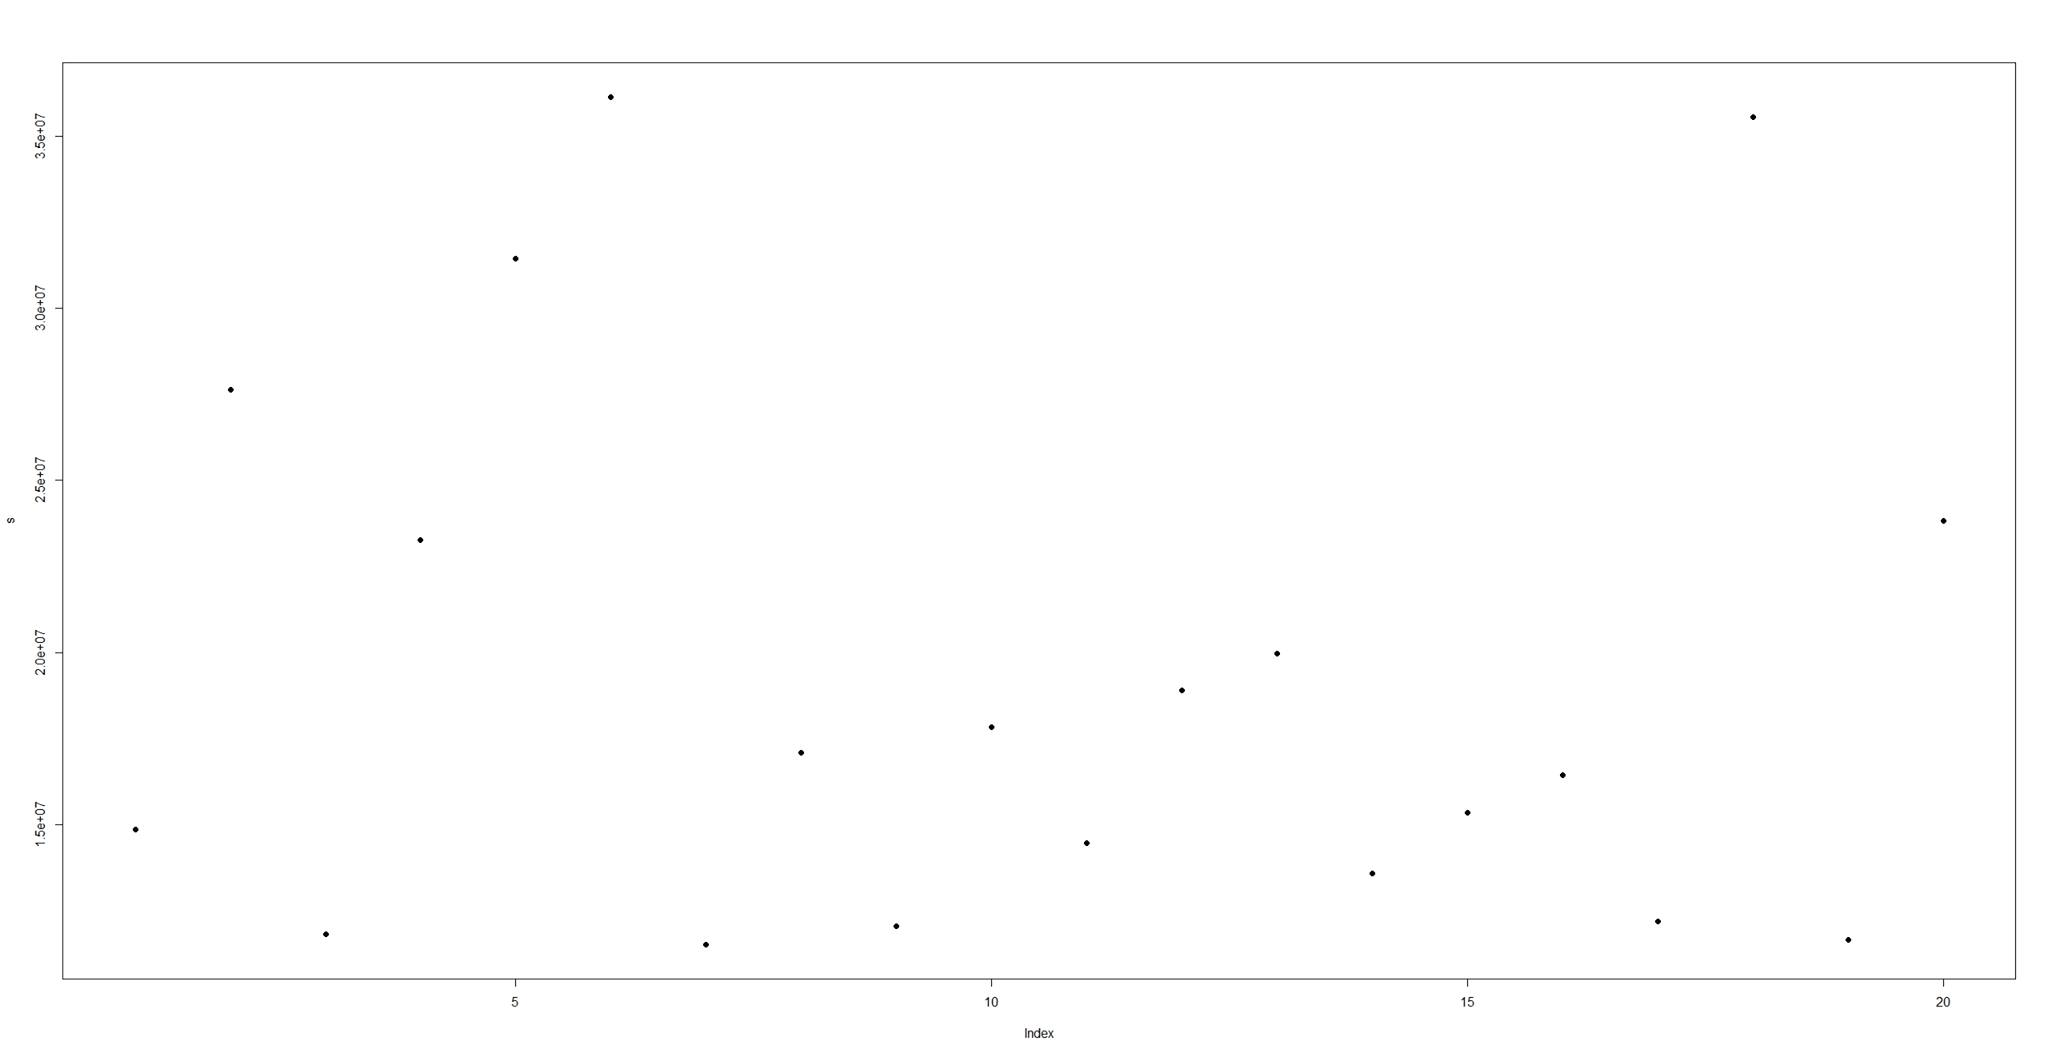
\includegraphics[width=0.9\textwidth]{plot4.jpg}
        \captionof{figure}{$\sum_j s_{ij}$ for all Contestants}
      \end{center}

      Finally, if salient means contestants that are the most different (highest $\sum_j s_{ij}$) then they are contestants 6, 18, and 5, in that order.
  \end{enumerate}

  \textbf{Code Appendix:}

  \begin{lstlisting}[language=R, basicstyle=\scriptsize, breaklines=true]
    # Part 2.1
    library(png)

    n <- 20
    p <- 117300

    pca <- matrix(0, n, p)

    ## Pre process images
    for(i in 1:20) {
      name <- paste("./images/", i, ".png", sep="")
      p <- readPNG(name)
      p <- p[171:400, 206:375, ]
      pca[i,] <- c(p)
    }

    ## Eigendecomposition using S = XX'/n
    decomp <- eigen(pca%*%t(pca)/n)
    D <- diag(decomp$values)
    U <- decomp$vectors

    # Part 2.2

    ## Plot eigenvalues
    dev.new()
    plot(1:20, decomp$values, type="o", pch=19)

    ## Top 6 eigenfaces
    V <- t(pca)%*%U
    rescale <- function(x){(x-min(x))/(max(x)-min(x))}
    V <- rescale(V)

    eigenface <- array(rep(0, 230*170*3*6), dim=c(230,170,3,6))

    for(i in 1:6) {
      eigenface[1:230,1:170,1,i] = matrix(t(V)[i, 1:39100], 230, 170)
      eigenface[1:230,1:170,2,i] = matrix(t(V)[i, 39101:78200], 230, 170)
      eigenface[1:230,1:170,3,i] = matrix(t(V)[i, 78201:117300], 230, 170)
      writePNG(eigenface[,,,i], target = paste("./eigenface", i, ".png", sep=""))
    }

    ## i-th image to k-th eigenface
    nu <- matrix(0,6,20)
    means <- rowMeans(pca)
    pca_center <- pca
    ## center the pca matrix
    for (i in 1:length(means)){
      pca_center[i,] <- pca_center[i,]-means[i]
    }

    for(i in 1:20) {
      for(k in 1:6) {
        nu[k,i] = t(V)[k,]%*%(pca_center[i,])
      }
    }
    dev.new()
    plot(nu[1,], pch=19)
    dev.new()
    plot(nu[2,], pch=19)

    ## Pairwise similarity
    s <- matrix(0,20,20)
    for(i in 1:20) {
      for(j in 1:20) {
        s[i,j] = sum((nu[,i] - nu[,j])^2)
      }
    }
    s <- rowSums(s)
    dev.new()
    plot(s, pch=19)
    print("Most salient contestants:")
    order(s, decreasing=T)[1:3]
  \end{lstlisting}
\end{answer}

\clearpage

\begin{exercise}
  In this problem, we will show that K-means algorithm can be derived as a limiting case of the EM algorithm for mixture of spherical Gaussians. That is, for the mixture model $p_{\psi} (x) = \sum_{j=1}^n p_{\theta_j} (x_j) \eta_j$, where $p_{\theta_j} (x_j)$ is the pdf of $\mathcal{N}(\theta_j, \sigma_j)$, start from the EM algorithm and find th appropriate settings for the E and M steps to reconstruct the K-means algorithm. Justify. (\textbf{Hint:} Calculate the limit $\lim_{\sigma_j^2 \rightarrow 0} \gamma_{ij}$)
\end{exercise}

\begin{answer}
  We have that the mixture for spherical Gaussians is
  \begin{gather*}
    \mathbb{P}_{\psi} (x) = \sum_{j=1}^n \mathbb{P}_{\theta_j} (x) \eta_j
  \end{gather*}
  Now, let $Y$ be the random variable of choosing Gaussian $j$, a categorical distribution, then the joint distribution is
  \begin{gather*}
    \mathbb{P}_{\psi} (x, y) = \sum_{j=1}^n \mathbb{P}_{\theta_j} (x) 1_{\{y = j\}} \eta_j
  \end{gather*}
  Then, from class, we derived the following E-step for this model
  \begin{gather*}
    \gamma_{ij}^{(t+1)} = \mathbb{P}_{\theta^{(t)}} (Y_i = j | X_i = x_i) = \frac{\mathbb{P}_{\theta_j^{(t)}}(x_i) \eta_j^{(t)}}{\sum_{k=1}^n \mathbb{P}_{\theta_k^{(t)}}(x_i) \eta_k^{(t)}}
  \end{gather*}
  Now, take $\sigma_j^2 \rightarrow 0$, then the above becomes the hard assignment
  \begin{gather*}
    \gamma_{ij} = \begin{cases}
      1 & \text{ if } \lVert x_i - \theta_j \rVert_2^2 < \lVert x_i - \theta_k \rVert_2^2, \ \forall \ j \neq k \\
      0 & \text{ otherwise}
    \end{cases}
  \end{gather*}
  Which is precisely the k-means step of assigning $x_i$ to the cluster with the closest center $\theta_j$. As the $\sigma_j$ disappear, the E-step only depends on $\theta_j$. Thus, we only need to update the $\theta_j$'s. The M-step becomes
  \begin{gather*}
    \theta_j^{(t+1)} = \frac{\sum_{i=1}^n \gamma_{ij}^{(t)} x_i}{\sum_{i=1}^n \gamma_{ij}^{(t)}} = \frac{\sum_{i: \gamma_{ij}^{(t)}=1} x_i}{\lvert \{ i : \gamma_{ij}^{(t)} = 1 \} \rvert}
  \end{gather*}
  Thus, the M-step calculates the new center of the cluster to be the average of all the points in the cluster. Thus, the E-step and M-step defined here is precisely the k-means algorithm.
\end{answer}

\clearpage

\begin{exercise}
  In this problem, we will derive the EM algorithm for the hidden Markov model (HMM). The HMM is defined as follows. Let $Z_1, \mathellipsis, Z_n \in \{1, \mathellipsis, k\}$ be a latent discrete Markov chain such that
  \begin{gather*}
    \mathbb{P}(Z_{i+1} = t | Z_i = s) = A_{st}, \text{ for any } i \geq 1
  \end{gather*}
  and $\mathbb{P}(Z_1 = j) = \eta_j$, where $\sum_{j=1}^{k} \eta_j = 1$. We observe $X_1, \mathellipsis, X_n \in \mathbb{R}^d$ where
  \begin{gather*}
    X_i | Z_i = j \sim \mathcal{N}(\mu_j, \Sigma_j), \text{ for any } i \geq 1
  \end{gather*}
  Our goal is to estimate $\psi = \{ A = [A_{st}]_{s,t=1}^k, \theta_j = (\mu_j, \Sigma_j), \eta = (\eta_1, \mathellipsis, \eta_k)^T \}$.
  \begin{enumerate}[label=\arabic*)]
    \item Derive the M-step for parameters. Show that the updating rule is
      \begin{align*}
        \eta_j &\leftarrow \frac{p_{\psi^{\text{old}}}(Z_1 = j | X_1, \mathellipsis, X_n)}{\sum_{\ell = 1}^k p_{\psi^{\text{old}}}(Z_1 = \ell | X_1, \mathellipsis, X_n)} \\
        A_{st} &\leftarrow \frac{\sum_{m=2}^n p_{\psi^{\text{old}}}(Z_m = t, Z_{m-1} = s | X_1, \mathellipsis, X_n)}{\sum_{\ell=1}^k \sum_{m=2}^n p_{\psi^{\text{old}}}(Z_m = \ell, Z_{m-1} = s | X_1, \mathellipsis, X_n)} \\
        \mu_j &\leftarrow \frac{\sum_{i=1}^n p_{\psi^{\text{old}}}(Z_i = j | X_1, \mathellipsis, X_n)X_i}{\sum_{i=1}^n p_{\psi^{\text{old}}}(Z_i = j | X_1, \mathellipsis, X_n)} \\
        \Sigma_j &\leftarrow \frac{\sum_{i=1}^n p_{\psi^{\text{old}}}(Z_i = j | X_1, \mathellipsis, X_n)(X_i - \bar{X})(X_i - \bar{X})^T}{\sum_{i=1}^n p_{\psi^{\text{old}}}(Z_i = j | X_1, \mathellipsis, X_n)}
      \end{align*}

    \item Derive the E-step to compute the conditional density $p_{\psi}(Z_i | X_1, \mathellipsis, X_n)$ for any $1 \leq j \leq k$. Let $\alpha(Z_i) = p(X_1, \mathellipsis, X_n, Z_i)$ and $\beta(Z_i) = p(X_{i+1}, \mathellipsis, X_n | Z_i)$. Show that
      \begin{gather*}
        p_{\psi}( Z_i | X_1, \mathellipsis, X_n) \propto \alpha(Z_i) \beta(Z_i) \text{ where } \\
        \alpha(Z_i) = p_{\psi}( X_i | Z_i) \sum_{Z_{i-1}} \alpha(Z_{i-1}) p_{\psi}( Z_i | Z_{i-1}) \\
        \beta(Z_i) = \sum_{Z_{i+1}} \beta(Z_{i+1}) p_{\psi}( X_{i+1} | Z_{i+1}) p_{\psi}( Z_{i+1} | Z_i)
      \end{gather*}
  \end{enumerate}
\end{exercise}

\clearpage

\begin{answer}
  \leavevmode
  \begin{enumerate}[label=\arabic*)]
    \item First, let us write the joint probability
      \begin{align*}
        & \mathbb{P}_{\psi} (Z_1, \mathellipsis, Z_n, X_1, \mathellipsis, X_n) \\
        &= \mathbb{P}_{\psi} (X_n | Z_1, \mathellipsis, Z_n, X_1, \mathellipsis, X_{n-1}) \cdot \\
        &\quad \mathbb{P}_{\psi} (Z_n | Z_1, \mathellipsis, Z_{n-1}, X_1, \mathellipsis, X_{n-1}) \cdot \\
        &\quad \mathbb{P}_{\psi} (Z_1, \mathellipsis, Z_{n-1}, X_1, \mathellipsis, X_{n-1}) \\
        &= \mathbb{P}_{\psi} (X_n | Z_n) \cdot \mathbb{P}_{\psi} (Z_n | Z_{n-1}) \cdot \mathbb{P}_{\psi} (Z_1, \mathellipsis, Z_{n-1}, X_1, \mathellipsis, X_{n-1})
      \end{align*}
      Where we used the Markov property in the last step. Applying the same result recursively yields
      \begin{gather*}
        \mathbb{P}_{\psi} (Z_1, \mathellipsis, Z_n, X_1, \mathellipsis, X_n) = \mathbb{P}_{\psi} (X_1 | Z_1) \mathbb{P}_{\psi} (Z_1) \prod_{i=2}^n \mathbb{P}_{\psi} (X_i | Z_i) \mathbb{P}_{\psi} (Z_i | Z_{i-1})
      \end{gather*}
      Which the above is the definition of the likelihood. Now, we note that
      \begin{gather*}
        X_i | Z_i = j \sim \mathcal{N}(\mu_j, \Sigma_j) \\
        \implies \mathbb{P}_{\psi} (X_i | Z_i) = \sum_{j=1}^k \phi_{\mu_j, \Sigma_j}(X_i) 1_{\{ Z_i = j \}} \\
        \mathbb{P}_{\psi} (Z_i | Z_{i-1}) = \sum_{j=1}^k \sum_{\ell=1}^k A_{j \ell} 1_{\{Z_{i-1} = j\}} 1_{\{Z_i = \ell\}} \ \forall \ i \geq 2 \\
        \mathbb{P}_{\psi} (Z_1) = \sum_{j=1}^k \eta_j 1_{\{Z_1 = j\}}
      \end{gather*}
      Thus, the log-likelihood becomes
      \begin{gather*}
        \ell_{\psi}(X,Z) = \sum_{i=2}^n \left( \sum_{j=1}^k \log \phi_{\mu_j, \Sigma_j}(X_i) 1_{\{ Z_i = j \}} + \sum_{j=1}^k \sum_{\ell=1}^k \log A_{j \ell} 1_{\{Z_{i-1} = j\}} 1_{\{Z_i = \ell\}} \right) \\
        + \sum_{j=1}^k \log \phi_{\mu_j, \Sigma_j}(X_1) 1_{\{ Z_1 = j \}} + \sum_{j=1}^k \log \eta_j 1_{\{Z_1 = j\}}
      \end{gather*}
      Now, we compute the E-step
      \begin{gather*}
        \mathbb{E} [\ell_{\psi} (X,Z) | X] = \sum_{i=2}^n \Big( \sum_{j=1}^k \log (\phi_{\mu_j, \Sigma_j}(X_i)) \mathbb{P}_{\psi^{(old)}} (Z_i = j | X_1, \mathellipsis, X_n ) \\
        + \sum_{j=1}^k \sum_{\ell=1}^k \log (A_{j \ell}) \mathbb{P}_{\psi^{(old)}} (Z_{i-1} = j, Z_i = \ell | X_1, \mathellipsis, X_n ) \Big) \\
        + \sum_{j=1}^k \log (\phi_{\mu_j, \Sigma_j}(X_1)) \mathbb{P}_{\psi^{(old)}} (Z_1 = j | X_1, \mathellipsis, X_n ) \\
        + \sum_{j=1}^k \log (\eta_j) \mathbb{P}_{\psi^{(old)}} (Z_1 = j | X_1, \mathellipsis, X_n )
      \end{gather*}
      Now we do the M-step and maximize according to each parameter. Note that we have set up the equation so that we can maximize individual sums as the sums only depend on one set of parameters at a time. Let's start with $\eta_j$. We have the constraint that $\sum_{j=1}^k \eta_j = 1$. Using a Lagrange multipler, the first order condition is
      \begin{gather*}
        \frac{\mathbb{P}_{\psi^{(old)}} (Z_1 = j | X_1, \mathellipsis, X_n )}{\eta_j} = \lambda, \quad \forall \ j
      \end{gather*}
      By our constraint, $\lambda = \sum_{j = 1}^k \mathbb{P}_{\psi^{(old)}} (Z_1 = j | X_1, \mathellipsis, X_n )$, thus
      \begin{gather*}
        \eta_j \leftarrow \frac{\mathbb{P}_{\psi^{\text{old}}}(Z_1 = j | X_1, \mathellipsis, X_n)}{\sum_{\ell = 1}^k \mathbb{P}_{\psi^{\text{old}}}(Z_1 = \ell | X_1, \mathellipsis, X_n)}
      \end{gather*}
      Similarly, for $A_{j \ell}$, we get the first order condition
      \begin{gather*}
        \frac{\sum_{i=2}^n \mathbb{P}_{\psi^{(old)}} (Z_{i-1} = j , Z_i = \ell| X_1, \mathellipsis, X_n )}{A_{j \ell}} = \lambda_j, \quad \forall \ j, \ell
      \end{gather*}
      Again, due to transition probabilities summing up to one,
      \begin{gather*}
        \lambda_j = \sum_{m=1}^k \sum_{i=2}^n \mathbb{P}_{\psi^{(old)}} (Z_{i-1} = j , Z_i = m | X_1, \mathellipsis, X_n )
      \end{gather*}
      Thus, the update rule is
      \begin{gather*}
        A_{st} \leftarrow \frac{\sum_{m=2}^n \mathbb{P}_{\psi^{\text{old}}}(Z_m = t, Z_{m-1} = s | X_1, \mathellipsis, X_n)}{\sum_{\ell=1}^k \sum_{m=2}^n \mathbb{P}_{\psi^{\text{old}}}(Z_m = \ell, Z_{m-1} = s | X_1, \mathellipsis, X_n)}
      \end{gather*}
      Now, we get to the parameters $\mu_j$ and $\Sigma_j$. We have that we want to maximize the following
      \begin{gather*}
        \sum_{i=1}^n \sum_{j=1}^k \log (\phi_{\mu_j, \Sigma_j}(X_i)) \mathbb{P}_{\psi^{(old)}} (Z_i = j | X_1, \mathellipsis, X_n)
      \end{gather*}
      However, we note that this is the same thing we maximize for the Gaussian mixture model updates which we did in class. Thus, we have the two last update rules
      \begin{align*}
        \mu_j &\leftarrow \frac{\sum_{i=1}^n \mathbb{P}_{\psi^{\text{old}}}(Z_i = j | X_1, \mathellipsis, X_n)X_i}{\sum_{i=1}^n \mathbb{P}_{\psi^{\text{old}}}(Z_i = j | X_1, \mathellipsis, X_n)} \\
        \Sigma_j &\leftarrow \frac{\sum_{i=1}^n \mathbb{P}_{\psi^{\text{old}}}(Z_i = j | X_1, \mathellipsis, X_n)(X_i - \bar{X})(X_i - \bar{X})^T}{\sum_{i=1}^n \mathbb{P}_{\psi^{\text{old}}}(Z_i = j | X_1, \mathellipsis, X_n)}
      \end{align*}

    \item The first relation results from
      \begin{align*}
        \mathbb{P}_{\psi} (Z_i | X_1, \mathellipsis, X_n) &= \frac{\mathbb{P}_{\psi}(Z_i, X_1, \mathellipsis, X_n)}{\mathbb{P}_{\psi}(X_1, \mathellipsis, X_n)} \\
        &\propto \mathbb{P}_{\psi}(Z_i, X_1, \mathellipsis, X_n) \\
        &\propto \mathbb{P}_{\psi}(X_{i+1}, \mathellipsis, X_n | Z_i, X_1, \mathellipsis, X_i) \mathbb{P}_{\psi}(Z_i, X_1, \mathellipsis, X_i) \\
        &\propto \mathbb{P}_{\psi}(X_{i+1}, \mathellipsis, X_n | Z_i) \mathbb{P}_{\psi}(Z_i, X_1, \mathellipsis, X_i) \\
        &\propto \beta(Z_i) \alpha(Z_i)
      \end{align*}
      Now, we show the recursive relation of $\alpha(Z_i)$
      \begin{align*}
        \alpha(Z_i) &= \mathbb{P}_{\psi}(Z_i, X_1, \mathellipsis, X_i) \\
        &= \sum_{j=1}^k \mathbb{P}_{\psi}(Z_{i-1} = j, Z_i, X_1, \mathellipsis, X_i) \\
        &= \sum_{j=1}^k \mathbb{P}_{\psi}(X_i | Z_{i-1} = j, Z_i, X_1, \mathellipsis, X_{i-1}) \mathbb{P}_{\psi}(Z_{i-1} = j, Z_i, X_1, \mathellipsis, X_{i-1})
      \end{align*}
      Using the Markov property
      \begin{align*}
        &= \sum_{j=1}^k \mathbb{P}_{\psi}(X_i | Z_i) \mathbb{P}_{\psi}(Z_{i-1} = j, Z_i, X_1, \mathellipsis, X_{i-1}) \\
        &= \mathbb{P}_{\psi}(X_i | Z_i) \sum_{j=1}^k \mathbb{P}_{\psi}(Z_i | Z_{i-1} = j, X_1, \mathellipsis, X_{i-1}) \mathbb{P}_{\psi}(Z_{i-1} = j, X_1, \mathellipsis, X_{i-1}) \\
        &= \mathbb{P}_{\psi}(X_i | Z_i) \sum_{j=1}^k \mathbb{P}_{\psi}(Z_i | Z_{i-1} = j) \alpha(Z_{i-1} = j) \\
        &= \mathbb{P}_{\psi}(X_i | Z_i) \sum_{Z_{i-1}}\mathbb{P}_{\psi}(Z_i | Z_{i-1}) \alpha(Z_{i-1})
      \end{align*}
      Now, for $\beta(Z_i)$,
      \begin{align*}
        \beta(Z_i) &= \mathbb{P}_{\psi}(X_{i+1}, \mathellipsis, X_n | Z_i) \\
        &= \sum_{j=1}^k \mathbb{P}_{\psi}(X_{i+1}, \mathellipsis, X_n, Z_{i+1} = j | Z_i) \\
        &= \sum_{j=1}^k \mathbb{P}_{\psi}(X_{i+1}, \mathellipsis, X_n | Z_i, Z_{i+1} = j) \mathbb{P}_{\psi}(Z_{i+1} = j | Z_i)
      \end{align*}
      Using the Markov property
      \begin{align*}
        &= \sum_{j=1}^k \mathbb{P}_{\psi}(X_{i+1}, \mathellipsis, X_n | Z_{i+1} = j) \mathbb{P}_{\psi}(Z_{i+1} = j | Z_i) \\
        &= \sum_{j=1}^k \Big( \mathbb{P}_{\psi}(X_{i+2}, \mathellipsis, X_n | Z_{i+1} = j, X_{i+1}) \mathbb{P}_{\psi}(X_{i+1} | Z_{i+1} = j) \\
        &\quad\quad\quad \mathbb{P}_{\psi}(Z_{i+1} = j | Z_i) \Big) \\
        &= \sum_{j=1}^k \beta(Z_{i+1} = j) \mathbb{P}_{\psi}(X_{i+1} | Z_{i+1} = j) \mathbb{P}_{\psi}(Z_{i+1} = j | Z_i) \\
        &= \sum_{Z_{i+1}} \beta(Z_{i+1}) \mathbb{P}_{\psi}(X_{i+1} | Z_{i+1}) \mathbb{P}_{\psi}(Z_{i+1} | Z_i)
      \end{align*}
  \end{enumerate}
\end{answer}

\clearpage

\begin{exercise}
  In this problem, we study the EM algorithm for the probabilistic PCA model. We consider the model $X = WZ + \epsilon$, where $Z \sim \mathcal{N}(0, I_q)$ is the latent variable and $\epsilon \sim \mathcal{N}(0, \sigma^2 I_d)$ is independent of $Z$. The matrix $W \in \mathbb{R}^{d \times q}$ is the linear transform matrix, where $q < d$. Suppose we observe i.i.d. data $X_1, \mathellipsis, X_n$ from this model, where $d < n$. Our goal is to estimate $W$ and $\sigma^2$ by EM algorithm.
  \begin{enumerate}[label=\arabic*)]
    \item What is the conditional distribution of $Z | X$?
    \item (Identifiability condition) Suppose $X = WZ + \epsilon$ and $\tilde{X} = VZ + \epsilon'$ both follow the probabilistic PCA model for $\epsilon \sim \mathcal{N}(0, \sigma^2 I_d)$ and $\epsilon \sim \mathcal{N}(0, \sigma'^2 I_d)$. If $X \stackrel{d}{=} \tilde{X}$, prove that $\sigma = \sigma'$ and there exists an orthogonal matrix $Q \in \mathbb{R}^{q \times q}$ such that $W = VQ$.
    \item Suppose $\sigma^2$ is known and the minimum eigenvalue of the sample covariance of $\{ X_i \}_{i=1}^n$ is larger than $\sigma^2$. What is the maximum likelihood estimator of $W$? (\textbf{Hint 1:} Consider the stationary points of the log-likelihood of the model first. \textbf{Hint 2:} Plug the singular decomposition of $W$ into the equation derived by Hint 1 and prove the general formulation of MLE of $W$. \textbf{Hint 3:} By the indentifiability in the previous question, the MLE of $W$ should be defined up to an orthogonal matrix.)
    \item Suppose the minimum eigenvalue of the sample covariance of $\{ X_i \}_{i=1}^n$ is larger than $\sigma^2$. What is the maximum likelihood estimator of $W$ and $\sigma^2$? (\textbf{Hint:} Use the result in the previous problem.)
    \item Write down the EM algoirthm to estimate both $W$ and $\sigma^2$. Show your work to get full credit.
  \end{enumerate}
\end{exercise}

\begin{answer}
  \leavevmode
  \begin{enumerate}[label=\arabic*)]
    \item Let us treat $(X,Z)$ as a joint Gaussian vector. $X$ is Gaussian as it is a linear combination of Gaussians. Now, we can treat this pair as being distributed as
      \begin{gather*}
        (X,Z) \sim \mathcal{N} \left( \begin{bmatrix} \mu_X \\ \mu_Z \end{bmatrix}, \begin{bmatrix} \Sigma_{XX} & \Sigma_{XZ} \\ \Sigma_{ZX} & \Sigma_{ZZ} \end{bmatrix} \right)
      \end{gather*}
      We know that $\mu_Z = 0$ and this implies that $\mu_X = 0$ as $\epsilon$ has 0 mean. Also given is $\Sigma_{ZZ} = I_q$. Now, we compute $\Sigma_{XX}$.
      \begin{gather*}
        \Sigma_{XX} = \mathbb{E}[X X^T] = \mathbb{E}[(WZ + \epsilon)(WZ + \epsilon)^T] \\
        = \mathbb{E}[WZZ^TW^T + WZ \epsilon^T + \epsilon Z^T W^T + \epsilon \epsilon^T]
      \end{gather*}
      Using the fact that $\epsilon \independent X$, the two middle terms are 0,
      \begin{align*}
        &= W \mathbb{E}[ZZ^T] W^T + \mathbb{E}[\epsilon \epsilon^T] \\
        &= W I_q W^T + \sigma^2 I_d \\
        &= W W^T + \sigma^2 I_d
      \end{align*}
      The covariance term is
      \begin{gather*}
        \Sigma_{XZ} = \mathbb{E}[X Z^T] = \mathbb{E}[(WZ + \epsilon) Z^T] \stackrel{X \independent \epsilon}{=} \mathbb{E}[WZ Z^T] = W
      \end{gather*}
      Lastly, $\Sigma_{ZX} = \Sigma_{XZ}^T$. Now we know all the means and covariances, we can use the formula for conditional Gaussians which yields
      \begin{gather*}
        Z | X \sim \mathcal{N}(W^T (W W^T + \sigma^2 I_d)^{-1} X, I_q - W^T (W W^T + \sigma^2 I_d)^{-1} W )
      \end{gather*}

    \item As we have $X \stackrel{d}{=} \tilde{X}$, then their variances must be equal. Then we must have
      \begin{gather*}
        W W^T + \sigma^2 I_d = V V^T + \sigma'^2 I_d
      \end{gather*}
      Now, since $W W^T$ and $V V^T$ are symmetric, they have diagonalizations
      \begin{gather*}
        W W^T = P \Lambda_W P^T \\
        V V^T = P' \Lambda_V P'^T
      \end{gather*}
      Thus, we have
      \begin{gather*}
        P (\Lambda_W + \sigma^2 I_d) P^T = P' (\Lambda_V + \sigma'^2 I_d) P'^T
      \end{gather*}
      Since, $q < d$, the nullspace of $W$ and $V$ is not empty. Thus, $\Lambda_W$ and $\Lambda_V$ have a 0 eigenvalue. This means that the minimal eigenvalue for $\Lambda_W + \sigma^2 I_d$ and $\Lambda_V + \sigma'^2 I_d$ are $\sigma$ and $\sigma'$ respectively. Thus we must have $\sigma = \sigma'$. Furthermore, by the same reasoning, with $\sigma = \sigma'$, all eigenvalues must be the same. If all the eigenvalue must be the same, then the equation above dictates that $P = P'$ and so they have the same eigendecomposition. Thus, by their SVD, we have
      \begin{gather*}
        W = P \Sigma_W  U \\
        V = P \Sigma_V U'
      \end{gather*}
      Where $P$ is the same in both as their decomposition from above is identical. We must also have $\Sigma_W = \Sigma_V$ from above. Both $U$ and $U'$ are orthogonal as it is a SVD and so there exists orthogonal $Q$ with $U = U' Q$. So we conclude that the same $Q$ also yields $W = VQ$.

    \item Recall that $X \sim \mathcal{N} (0, W W^T + \sigma^2 I_d)$. Then we have that the log-likelihood is
      \begin{gather*}
        \ell (X) = \sum_{i=1}^n \log \phi_{0, W W^T + \sigma^2 I_d} (X_i) \\
        = -\frac{nd}{2} \log(2 \pi) - \frac{n}{2} \log \lvert W W^T + \sigma^2 I_d \rvert - \frac{n}{2} \sum_{i=1}^n X_i^T (W W^T + \sigma^2 I_d)^{-1} X_i \\
        = -\frac{nd}{2} \log(2 \pi) - \frac{n}{2} \log \lvert W W^T + \sigma^2 I_d \rvert \\
        - \frac{n}{2} \text{Tr} \left( \sum_{i=1}^n (X_i X_i^T)(W W^T + \sigma^2 I_d)^{-1} \right)
      \end{gather*}
      Now, letting $\hat{\Sigma} = \frac{1}{n} \sum_{i=1}^n (X_i X_i^T$, taking the matrix differentiation of the above yields, after a long and arduous process,
      \begin{gather*}
        \frac{\partial \ell}{\partial W} = n ( (W W^T + \sigma^2 I_d)^{-1} \hat{\Sigma} (W W^T + \sigma^2 I_d)^{-1} W - (W W^T + \sigma^2 I_d)^{-1} W )
      \end{gather*}
      Which means the stationary points are
      \begin{gather*}
        \hat{\Sigma} (W W^T + \sigma^2 I_d)^{-1} W = W
      \end{gather*}
      We ignore the trivial solution $W = 0$. Following the hint, let $W = U \Sigma V^T$ be the SVD decomposition. We plug this into the above.
      \begin{gather*}
        \hat{\Sigma} (U \Sigma^2 U^T + \sigma^2 I_d)^{-1} U \Sigma V^T = U \Sigma V^T
      \end{gather*}
      Post multiplying by $V$, and since the inverted term is diagonal, and $U \Sigma^2 U^T = \Sigma^2$,
      \begin{gather*}
        \hat{\Sigma} U \Sigma = U (U \Sigma^2 U^T+ \sigma^2 I_d) \Sigma
      \end{gather*}
      Now, take an eigenvector of $U$, says $u_i$, such that $\sigma_i \neq 0$ (one of the elements of $\Sigma$), then
      \begin{gather*}
        \hat{\Sigma} u_i = (\sigma_i^2 + \sigma^2) u_i
      \end{gather*}
      So $u_i$ is an eigenvector of $\hat{\Sigma}$ with eigenvalue $\lambda_i = \sigma_i^2 + \sigma^2$. Thus, the stationary points of the MLE are
      \begin{gather*}
        W = U \Sigma V^T
      \end{gather*}
      Where $U$ is picked such that the first $r$ columns are eigenvectors of $\hat{\Sigma}$, the rest are arbitrary. Plugging this back into the log-likelihood, using the fact that the determinant is the product of eigenvalues, and the trace is the sum of eigenvalues,
      \begin{gather*}
        \ell(X) \propto - \log \lvert W W^T + \sigma^2 I_d \rvert - \text{Tr} \left(\hat{\Sigma} (W W^T + \sigma^2 I_d)^{-1} \right) \\
        = - \log \lvert U \Sigma^2 U^T + \sigma^2 I_d \rvert - \text{Tr} \left( \hat{\Sigma} (U \Sigma^2 U^T + \sigma^2 I_d)^{-1} \right) \\
        = - \sum_{i = 1}^r \log(\lambda_i) - \sum_{i = r+1}^d \log(\sigma^2) - \sum_{i = 1}^r 1 - \sum_{i = r+1}^d \frac{\lambda_i}{\sigma^2}
      \end{gather*}
      Where the trace simplifies to the above because $\hat{\Sigma} = U \text{diag}(\lambda_1 + \mathellipsis, \lambda_r, \sigma^2, \mathellipsis, \sigma^2) U^T$. Therefore, we must pick a suitable $r$ that maximizes this. Noting that $-\log(\lambda_i) + \log(\sigma^2) \geq 1 - \frac{\lambda_i}{\sigma^2}$ from log inequalities, we want to maximize $r$ to maximize likelihood, thus $r = q$. Then pick $W$ to be the SVD with $U$ having $q$ eigenvector columns of $\hat{\Sigma}$.

    \item The MLE for $W$ does not change from the last part. From the previous part, we get that the log likelihood is
      \begin{gather*}
        \ell(X) \propto - \sum_{i = 1}^q \log(\lambda_i) - \sum_{i = q+1}^d \log(\sigma^2) - \sum_{i = 1}^q 1 - \sum_{i = q+1}^d \frac{\lambda_i}{\sigma^2}
      \end{gather*}
      The first order condition for this is
      \begin{gather*}
        \frac{\partial \ell}{\partial \sigma^2} = - \sum_{i = q+1}^d \frac{1}{\sigma^2} + \sum_{i = q+1}^d \frac{\lambda_i}{\sigma^4} = 0 \\
        \implies \sigma^2 = \frac{1}{d-q} \sum_{i = q+1}^d \lambda_i
      \end{gather*}
      Which is the MLE for $\sigma$.

    \item Recall the joint density of $(X, Z) \sim \mathcal{N} \left( \begin{bmatrix} 0 \\ 0 \end{bmatrix}, \begin{bmatrix} \sigma^2 I_d + W W^T & W^T \\ W & I_q \end{bmatrix} \right)$. Now, the log-likelihodd of a Gaussian is
      \begin{gather*}
        \ell_{\psi}(X, Z) \propto - n \log \lvert \Sigma \rvert - \sum_{i=1}^n \begin{bmatrix} X_i^T & Z_i^T \end{bmatrix} \Sigma^{-1} \begin{bmatrix} X_i \\ Z_i \end{bmatrix}
      \end{gather*}
      Where $\Sigma = \begin{bmatrix} \sigma^2 I_d + W W^T & W^T \\ W & I_q \end{bmatrix}$. Now note that
      \begin{gather*}
        \Sigma = \begin{bmatrix} I_d & W^T \\ 0 & I_q \end{bmatrix} \begin{bmatrix} \sigma^2 I_d & 0 \\ 0 & I_q \end{bmatrix} \begin{bmatrix} I_d & 0 \\ W & I_q \end{bmatrix}
      \end{gather*}
      Thus,
      \begin{align*}
        \det \Sigma &= \det \begin{bmatrix} I_d & W^T \\ 0 & I_q \end{bmatrix} \cdot \det \begin{bmatrix} \sigma^2 I_d & 0 \\ 0 & I_q \end{bmatrix} \cdot \det \begin{bmatrix} I_d & 0 \\ W & I_q \end{bmatrix} \\
        &= 1 \cdot \sigma^{2^d} \cdot 1 \\
        &= \sigma^{2^d}
      \end{align*}
      Deriving the inverse from the above is simple, we just find the inverse for the simpler matrices and reverse the order,
      \begin{gather*}
        \Sigma^{-1} = \begin{bmatrix} I_d & 0 \\ -W & I_q \end{bmatrix} \begin{bmatrix} \frac{1}{\sigma^2} I_d & 0 \\ 0 & I_q \end{bmatrix} \begin{bmatrix} I_d & -W^T \\ 0 & I_q \end{bmatrix}
      \end{gather*}
      This makes the log-likelihood become
      \begin{align*}
        \ell_{\psi} (X, Z) \propto &- n d \log \sigma^2 \\
        &- \sum_{i=1}^n \begin{bmatrix} X_i^T & Z_i^T \end{bmatrix} \begin{bmatrix} I_d & 0 \\ -W & I_q \end{bmatrix} \begin{bmatrix} \frac{1}{\sigma^2} I_d & 0 \\ 0 & I_q \end{bmatrix} \begin{bmatrix} I_d & -W^T \\ 0 & I_q \end{bmatrix} \begin{bmatrix} X_i \\ Z_i \end{bmatrix} \\
        &= - n d \log \sigma^2 - \sum_{i=1}^n \begin{bmatrix} X_i^T - Z_i^T W & Z_i^T \end{bmatrix} \begin{bmatrix} \frac{1}{\sigma^2} I_d & 0 \\ 0 & I_q \end{bmatrix} \begin{bmatrix} X_i - W^T Z_i \\ Z_i \end{bmatrix} \\
        &= -n d \log \sigma^2 \\
        &+ \sum_{i=1}^n \frac{1}{\sigma^2} (X_i^T X_i - 2 X_i^T W Z_i + Z_i^T W^T W Z_i) + Z_i^T Z_i
      \end{align*}
      To do the E-step, we take conditional expectation on $X$
      \begin{align*}
        \mathbb{E}[ \ell_{\psi}(X,Z) | X] = &- n d \log \sigma^2 - \sum_{i=1}^n \frac{X_i^T X_i}{\sigma^2} \\
        &+ 2\sum_{i=1}^n \frac{\text{Tr}(X_i^T W \mathbb{E}_{\psi^{(\text{old})}}[Z_i | X_i])}{\sigma^2} \\
        &- \sum_{i=1}^n \frac{\text{Tr}(W \mathbb{E}_{\psi^{(\text{old})}}[Z_i Z_i^T | X_i] W^T)}{\sigma^2} \\
        &- \sum_{i=1}^n \mathbb{E}_{\psi^{(\text{old})}}[Z_i^T Z_i | X_i]
      \end{align*}
      Where the conditional expectations can be explicitly solved for using part 1). Now, we do the M-step. We use the fact that $\frac{\partial}{\partial X} \text{Tr} (AXB) = BA$ and $\frac{\partial}{\partial X} \text{Tr} (X B X^T) = X B^T + X B$. Thus, taking the derivative of the log-likelihood with respect to $W$ and setting to 0 yields
      \begin{gather*}
        \sum_{i=1}^n 2 X_i \mathbb{E}_{\psi^{(\text{old})}}[Z_i | X_i]^T - W \mathbb{E}_{\psi^{(\text{old})}}[Z_i Z_i^T | X_i] + W \mathbb{E}_{\psi^{(\text{old})}} [Z_i Z_i^T | X_i]^T = 0
      \end{gather*}
      But, $\mathbb{E}_{\psi^{(\text{old})}} [Z_i Z_i^T | X_i]$ is symmetric, so
      \begin{gather*}
        \sum_{i=1}^n X_i \mathbb{E}_{\psi^{(\text{old})}}[Z_i | X_i]^T = W \sum_{i=1}^n \mathbb{E}_{\psi^{(\text{old})}}[Z_i Z_i^T | X_i] \\
        \implies W \leftarrow \left( \sum_{i=1}^n X_i \mathbb{E}_{\psi^{(\text{old})}}[Z_i | X_i]^T \right) \left( \sum_{i=1}^n \mathbb{E}_{\psi^{(\text{old})}}[Z_i Z_i^T | X_i] \right)^{-1}
      \end{gather*}
      Finally, estimate $\sigma^2$ by maximizing the E-step w.r.t. $\sigma$, first order conditions are
      \begin{align*}
        0 = &-\frac{n d}{\sigma^2} + \frac{1}{\sigma^4} \sum_{i=1}^n X_i^T X_i \\
        &- \frac{2}{\sigma^4} \text{Tr}(X_i^T W \mathbb{E}_{\psi^{(\text{old})}}[Z_i | X_i]) + \frac{1}{\sigma^4} \sum_{i=1}^n \text{Tr}(W \mathbb{E}_{\psi^{(\text{old})}}[Z_i Z_i^T | X_i] W^T) \\
        \implies \sigma^2 &\leftarrow \frac{1}{n d} \sum_{i=1}^n X_i^T X_i \\
        &- \frac{2}{n d} \text{Tr}(X_i^T W \mathbb{E}_{\psi^{(\text{old})}}[Z_i | X_i]) + \frac{1}{n d} \sum_{i=1}^n \text{Tr}(W \mathbb{E}_{\psi^{(\text{old})}}[Z_i Z_i^T | X_i] W^T)
      \end{align*}
  \end{enumerate}
\end{answer}

\end{document}